\documentclass{homework}
\usepackage{ctex}
\usepackage{bm}
\usepackage{makecell}
\usepackage[ruled,vlined]{algorithm2e}
\usepackage{booktabs}
\usepackage{multirow}
\usepackage{siunitx}
\usepackage{graphicx}
\usepackage{amsmath}
\usepackage{subcaption}
\usepackage{caption}
\newcommand{\bfx}{\mathbf{x}}
\newcommand{\bfg}{\mathbf{g}}
\newcommand{\bfH}{\mathbf{H}}
\newcommand{\bfd}{\mathbf{d}}
\author{李健宁}
\class{机器学习中的优化问题}
\date{\today}
\title{Homework 13}
% \address{Bayt El-Hikmah}

\graphicspath{{./media/}}

\begin{document} \maketitle

\question

\begin{sol}
与上一次作业不同的是$E$的更新使用上一轮的$Z$而非新更新的$Z$,以及一些参数的变化(如$\eta_D$)。

    引入拉格朗日乘子 \( Y_1 \in \mathbb{R}^{m \times n} \),\( Y_2 \in \mathbb{R}^{n \times 1} \),增广拉格朗日函数为:

\[
\begin{aligned}
\mathcal{L}(Z, E, Y_1, Y_2) = &\|Z\|_* + \lambda \|E\|_{2,1} + \langle Y_1, D - DZ - E \rangle + \frac{\beta}{2} \|D - DZ - E\|_F^2 \\
&+ \langle Y_2, Z^\top \mathbf{1} - \mathbf{1} \rangle + \frac{\beta}{2} \|Z^\top \mathbf{1} - \mathbf{1}\|_2^2
\end{aligned}
\]


\subsection*{更新 \( Z \)}

我们线性化增广拉格朗日中关于 \( Z \) 的二次项,得到以下更新:

\[
Z^{k+1} = \arg\min_Z \|Z\|_* + \frac{\beta_k}{2} \|Z - G^k\|_F^2
\]

其中:

\[
G^k = Z^k - \frac{1}{\eta_D} \left( D^\top (D Z^k + E^k - D) + \mathbf{1}(Z^{k\top} \mathbf{1} - \mathbf{1})^\top + \frac 1{\beta_k}D^\top Y_1^k + \frac 1{\beta_k}\mathbf{1} Y_2^{k^\top} \right)
\]

该子问题的解为奇异值软阈值:

\[
Z^{k+1} = \operatorname{SVT}_{1/\eta_D\beta_k}(G^k)
\]

\subsection*{更新 \( E \)}

对 \( E \) 的更新为:

\[
E^{k+1} = \arg\min_E \lambda \|E\|_{2,1} + \frac{\beta_k}{2} \left\| E - \left(D - D Z^{k+1} + \frac{1}{\beta_k} Y_1^k \right) \right\|_F^2
\]

这是 \( \ell_{2,1} \) 范数的近端问题,解为对每列进行缩放:

\[
E^{k+1}_{:,j} = \left[1 - \frac{1}{\beta_k\|R_{:,j}\|_2} \right]_+ R_{:,j}, \quad R = D - D Z^{k+1} + \frac{1}{\beta_k} Y_1^k
\]

\subsection*{更新拉格朗日乘子}

\[
\begin{aligned}
Y_1^{k+1} &= Y_1^k + \beta_k (D - D Z^{k+1} - E^{k+1}) \\
Y_2^{k+1} &= Y_2^k + \beta_k (Z^{k+1^\top} \mathbf{1} - \mathbf{1})
\end{aligned}
\]

\subsection*{自适应步长更新}

使用如下策略自适应更新 \( \beta_k \):

\[
\beta_{k+1} = \min(\rho \beta_k, \beta_{\max})
\]
$$
\rho= \begin{cases}\rho_0, & \text { if } \beta_k \max \left(\sqrt{\eta_D}\left\|\mathbf{x}_{k+1}-\mathbf{x}_k\right\|, \left\|\mathbf{y}_{k+1}-\mathbf{y}_k\right\|\right) /\|\mathbf{c}\|<\varepsilon_2 \\ 1, & \text { otherwise }\end{cases}
$$
\subsection*{收敛条件}
\[
\frac{\|DZ^k+E^k - D\|}{\|D\|}\le \epsilon_1,\, \text{or}
\max\left( \frac{\|D^k-D^{k-1}\|}{\|D\|}, \frac{\|E^k-E^{k-1}\|}{\|D\|} \right) < \epsilon_2
\]

\subsection*{数据实验}

参数选取上, \(\epsilon_1 = 10^{-6},\, \epsilon_2=10^{-5},\, \beta_0=\min(n,m)\epsilon_2 = 200\epsilon_2,\, \beta_{\max}=10^{10},\, \rho_0 = 1.9,\,\eta_D = 2.02\sigma^2_{\max}(\mathrm D) \),$\lambda = 0.1$,最大迭代次数5000次。最终实验结果如图\ref{4}
\begin{figure}[h]
    \centering
        \centering
        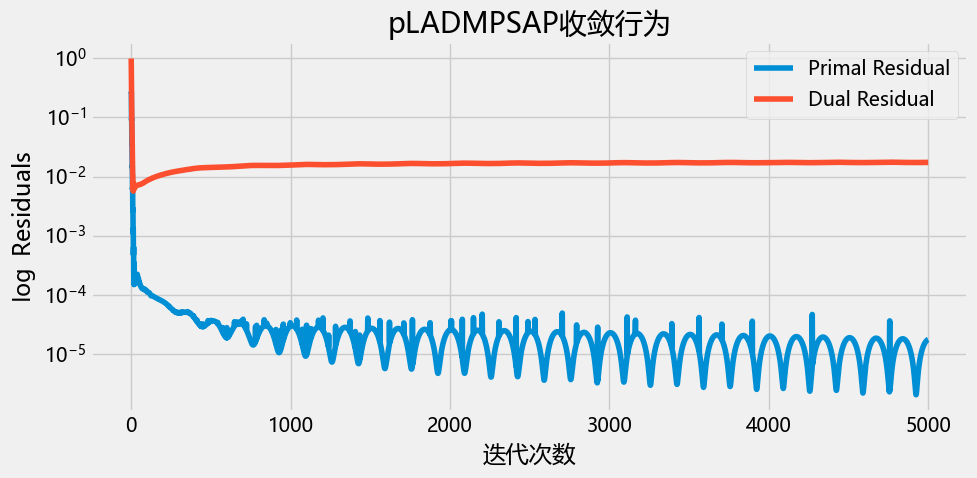
\includegraphics[width=0.8\linewidth]{4.png}
        \caption{LADMPSAP收敛行为}\label{4}
\end{figure}
\end{sol}

\question

\begin{sol}
    \[
\min_{\bar{\mathbf{w}} \in \mathbb{R}^d} \; \frac{1}{s} \sum_{i=1}^{s} \log\left(1 + \exp(-y_i \bar{\mathbf{w}}^\top \bar{\mathbf{x}}_i)\right)
\]
其中 $\bar{\mathbf{x}}_i \in \mathbb{R}^d$,$y_i \in \{-1, +1\}$。

\subsection*{梯度的Lipschitz常数}

逻辑损失的梯度
\[
\nabla f(\bar{\mathbf{w}}) = -\frac{1}{s} \sum_{i=1}^{s} y_i \bar{\mathbf{x}}_i \cdot \sigma(-y_i \bar{\mathbf{w}}^\top \bar{\mathbf{x}}_i)
\]
其中 $\sigma(z) = \frac{1}{1 + e^{-z}}$ 。

Hessian
\[
\nabla^2 f(\bar{\mathbf{w}}) = \frac{1}{s} \sum_{i=1}^s \sigma(y_i \bar{\mathbf{w}}^\top \bar{\mathbf{x}}_i)\left(1 - \sigma(y_i \bar{\mathbf{w}}^\top \bar{\mathbf{x}}_i)\right) \bar{\mathbf{x}}_i \bar{\mathbf{x}}_i^\top
\]

由于对任意实数 $z$ 有
\[
\sigma(z)(1 - \sigma(z)) \leq \frac{1}{4}
\]

可得 Hessian 的谱范数(最大特征值)满足:
\[
\|\nabla^2 f(\bar{\mathbf{w}})\| \leq \frac{1}{4s} \sum_{i=1}^s \|\bar{\mathbf{x}}_i\|^2 = \frac{1}{4s} \|\bar{\mathbf{X}}\|_F^2
\]

因此梯度 Lipschitz 常数满足:
\[
L_{\bar{\mathbf{w}}} \leq \frac{1}{4s} \|\bar{\mathbf{X}}\|_F^2
\]

\subsection*{pLADMPSAP推导}

引入局部变量 $\bar{\mathbf{w}}_i$和约束
\[
\bar{\mathbf{w}}_i = \bar{\mathbf{w}}, \quad \forall i=1,\dots,s
\]

优化问题变为
\[
\min_{\{\bar{\mathbf{w}}_i\}, \bar{\mathbf{w}}} \; \frac{1}{s} \sum_{i=1}^s \log\left(1 + \exp(-y_i \bar{\mathbf{w}}_i^\top \bar{\mathbf{x}}_i)\right) \quad \text{s.t.} \bar{\mathbf{w}}_i = \bar{\mathbf{w}},\, 1\le i \le s
\]

构造增广拉格朗日
\[
\mathcal{L} = \frac{1}{s} \sum_{i=1}^s \log\left(1 + \exp(-y_i \bar{\mathbf{w}}_i^\top \bar{\mathbf{x}}_i)\right) + \sum_{i=1}^s \left\langle \bm{\alpha}_i, \bar{\mathbf{w}}_i - \bar{\mathbf{w}} \right\rangle + \frac{\rho}{2} \sum_{i=1}^s \|\bar{\mathbf{w}}_i - \bar{\mathbf{w}}\|^2
\]

在第 $k$ 次迭代中,执行以下操作:

\begin{enumerate}
    \item 更新局部变量 $\bar{\mathbf{w}}_i^{k+1}$,使用梯度下降:
    \[
    \bar{\mathbf{w}}_i^{k+1} = \arg\min \left\{ \frac{1}{s} \log\left(1 + \exp(-y_i \bar{\mathbf{w}}_i^\top \bar{\mathbf{x}}_i)\right) + \langle \bm{\alpha}_i^k, \bar{\mathbf{w}}_i - \bar{\mathbf{w}}^k \rangle + \frac{\rho}{2} \|\bar{\mathbf{w}}_i - \bar{\mathbf{w}}^k\|^2 \right\}
    \]
    
    \item 更新全局变量 $\bar{\mathbf{w}}$:
    \[
    \bar{\mathbf{w}}^{k+1} = \frac{1}{s} \sum_{i=1}^s \left( \bar{\mathbf{w}}_i^{k+1} + \frac{1}{\rho} \bm{\alpha}_i^k \right)
    \]
    
    \item 更新拉格朗日乘子:
    \[
    \bm{\alpha}_i^{k+1} = \bm{\alpha}_i^k + \rho (\bar{\mathbf{w}}_i^{k+1} - \bar{\mathbf{w}}^{k+1})
    \]
\end{enumerate}

\subsection*{数据实验}

选取$s=30,d=20$,随机生成$X\in\mathrm{R}^{s\times d}$和$w\in\mathrm{R}^d$,$y = \text{sign}(Xw+\sigma \varepsilon), \sigma = 0.1,\varepsilon\sim N(0,1)$。最大迭代次数$10000$次。梯度下降方法学习率$0.1$,停止标准$\|\nabla f(x)\|\le10^{-6}$。pLADPSAP方法$\rho = 1.0$,停止标准$\|w_i-w\|\le 10^{-6}$。实验结果如图\ref{fig:2},GD收敛更快。

\begin{figure}[h]
    \centering
    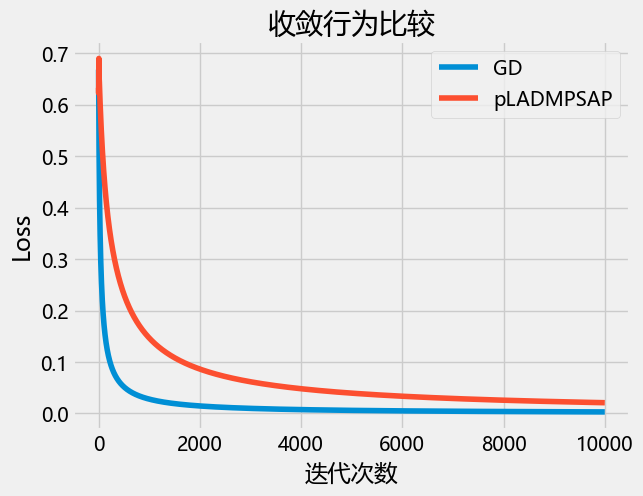
\includegraphics[width=0.5\linewidth]{2.png}
    \caption{收敛行为比较}
    \label{fig:2}
\end{figure}

\end{sol}



\question

\begin{sol}


\subsection*{固定 $\mathbf{D}$,更新 $\mathbf{X}$}

固定字典 $\mathbf{D}$ 后,$\mathbf{X}$ 的优化问题变为
\[
\min_{\mathbf{X}} \quad  \frac{1}{2} \|\mathbf{Y} - \mathbf{D}\mathbf{X}\|_F^2 + \lambda \|\mathbf{X}\|_1
\]

可以将其拆解为 $n$ 个独立的 Lasso 问题
\[
\min_{\mathbf{x}_i} \quad  \frac{1}{2} \|\mathbf{y}_i - \mathbf{D} \mathbf{x}_i\|_2^2 + \lambda \|\mathbf{x}_i\|_1, \quad \forall i = 1, \dots, n
\]

\subsection*{固定 $\mathbf{X}$,更新 $\mathbf{D}$}

此时优化目标变为
\[
\min_{\mathbf{D}} \quad \frac{1}{2} \|\mathbf{Y} - \mathbf{D} \mathbf{X}\|_F^2 \quad \text{s.t.} \quad  \|\mathbf{d}_i\|_2 = 1, \quad \forall i.
\]

忽略约束条件时,有闭式解
\[
\mathbf{D} = \mathbf{Y} \mathbf{X}^\top (\mathbf{X} \mathbf{X}^\top)^{-1}.
\]

为防止矩阵奇异,引入正则项,得
\[
\mathbf{D} = \mathbf{Y} \mathbf{X}^\top (\mathbf{X} \mathbf{X}^\top + \epsilon \mathbf{I})^{-1}.
\]

为了满足约束 $\|\mathbf{d}_i\|_2 = 1$,对每一列归一化
\[
\mathbf{d}_i \leftarrow \frac{\mathbf{d}_i}{\|\mathbf{d}_i\|_2}, \quad \forall i.
\]

\subsection*{实验参数选取}

参数选取上,$\lambda = 0.01$,最大迭代次数$500$次,为防止矩阵奇异引入的正则项系数$\epsilon = 10^{-3}$,Lasso问题使用\texttt{sklearn.linear\_model.Lasso}求解,最大迭代次数$1000$次。实验结果如图\ref{fig:1}。

\begin{figure}[h]
    \centering
    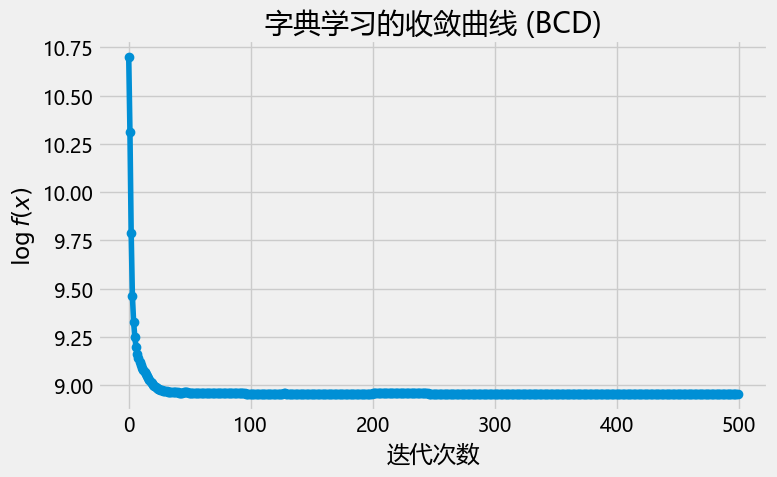
\includegraphics[width=0.5\linewidth]{1.png}
    \caption{收敛行为}
    \label{fig:1}
\end{figure}
\end{sol}

\question

\begin{sol}

\textbf{更新$\bm{A}$}

固定 $\bm{U}$ 和 $\bm{V}$,我们更新 $\bm{A}$ 的问题为:
\[
\min_{\bm{A}} \frac{1}{2} \left\| \bm{U}\bm{V}^\top - \bm{A} \right\|_F^2, \quad \text{s.t. } \mathcal{P}_\Omega(\bm{A}) = \mathcal{P}_\Omega(\bm{D}).
\]
该问题的解析解为:
\[
\bm{A} = \mathcal{P}_\Omega(\bm{D}) + \mathcal{P}_{\Omega^c}(\bm{U}\bm{V}^\top),
\]
即在观测位置保留原始数据,其余位置用当前的低秩估计补全。

\textbf{更新 $\bm{U}$}

固定 $\bm{A}$ 和 $\bm{V}$,我们更新 $\bm{U}$ 的问题为:
\[
\min_{\bm{U}} \frac{1}{2} \left\| \bm{U}\bm{V}^\top - \bm{A} \right\|_F^2.
\]
该问题的解析解为:
\[
\bm{U} = \bm{A} \bm{V} (\bm{V}^\top \bm{V})^{-1}.
\]

\textbf{更新 $\bm{V}$}

固定 $\bm{A}$ 和 $\bm{U}$,我们更新 $\bm{V}$ 的问题为:
\[
\min_{\bm{V}} \frac{1}{2} \left\| \bm{U}\bm{V}^\top - \bm{A} \right\|_F^2.
\]
该问题的解析解为:
\[
\bm{V} = \bm{A}^\top \bm{U} (\bm{U}^\top \bm{U})^{-1}.
\]

\textbf{正交化步骤}

为提升算法的数值稳定性,我们可在每轮迭代中对 $\bm{U}$ 或 $\bm{V}$ 进行 QR 正交化处理。例如:
\[
\bm{U} \leftarrow \bm{Q}, \quad \text{其中 } \bm{Q}\bm{R} = \text{QR分解}(\bm{U}).
\]

\textbf{实验设置}

根据题目要求随机生成相应的矩阵,数据实验结果如图\ref{fig:3}。能够看出,在经历相当多的迭代次数后,更新$U$后正交化的策略收敛。

\begin{figure}[h]
    \centering
    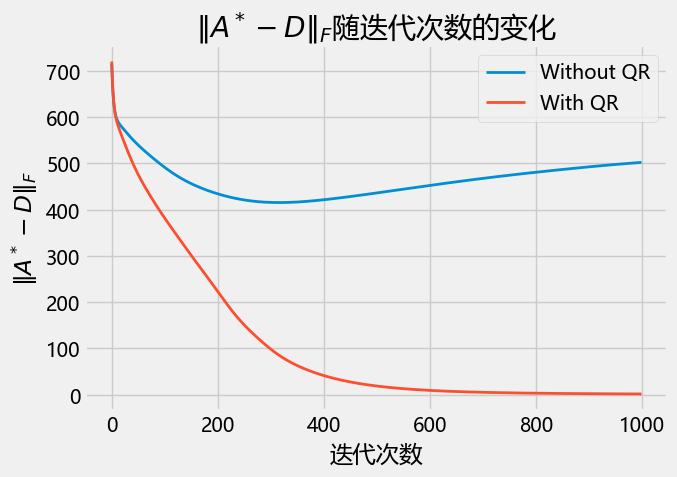
\includegraphics[width=0.5\linewidth]{3.png}
    \caption{$ \|A^* - D\|_F $随迭代次数的变化}
    \label{fig:3}
\end{figure}
\end{sol}

\question

\begin{sol}
    每轮迭代分为两步:

\begin{itemize}
  \item \textbf{Step 1:更新 $\boldsymbol{y}_i$}

  固定 $\boldsymbol{x}^{(k)}$,每个 $\boldsymbol{y}_i$ 独立优化
  \[
  \boldsymbol{y}_i^{(k+1)} = \operatorname{Proj}_{\mathcal{X}_i}(\boldsymbol{x}^{(k)})
  \]

  \item \textbf{Step 2:更新 $\boldsymbol{x}$}

  固定所有 $\boldsymbol{y}_i^{(k+1)}$,则有闭式解:
  \[
  \boldsymbol{x}^{(k+1)} = \frac{1}{m} \sum_{i=1}^m \boldsymbol{y}_i^{(k+1)}
  \]
\end{itemize}

\section{收敛性分析}

若所有集合 $\mathcal{X}_i$ 是非空闭凸集,且它们的交集非空,即
\[
\bigcap_{i=1}^m \mathcal{X}_i \neq \emptyset
\]
则上述算法生成的序列 $\boldsymbol{x}^{(k)}$ 将收敛到该交集中的一点。该点即为原始问题的最优解。

\textbf{数据实验}  \quad $m = 5$时,随机生成$5$个圆心在$[-3,3]^2$,半径为$3$的二维圆盘,生成若干次直至所有圆盘的交集不为空。初始点 $\boldsymbol{x}^{(0)}$ 从$[-20,20]^2$中产生,生成若干次直至该点不在所有圆盘的交集中,作为初始位置。运行 100 次迭代,记录收敛过程如图\ref{5}.

\begin{figure}[h]
    \centering
    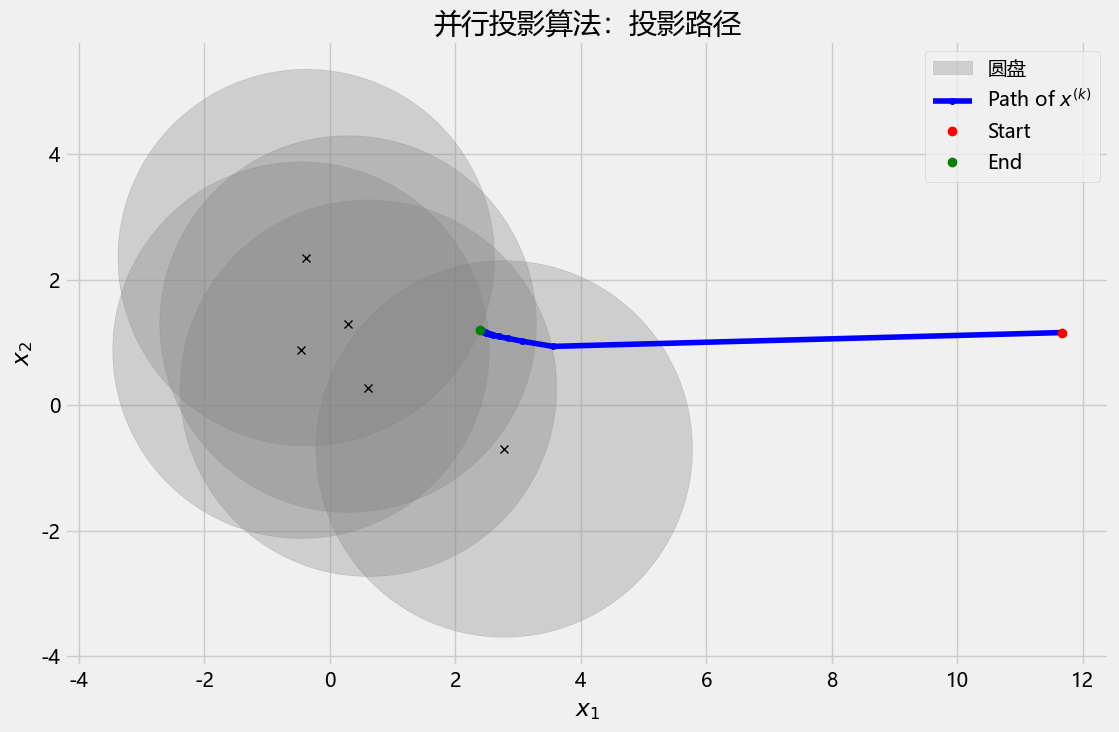
\includegraphics[width=0.5\linewidth]{5.png}
    \caption{投影路径}
    \label{5}
\end{figure}
\end{sol}

    % citations
% \bibliographystyle{plain}
% \bibliography{citations}

\end{document}
